\chapter{Data analysis and Event reconstruction}\label{section:Reconstruction}


\section{Data analysis}\label{sec:Data analysis}
\subsection{Event selection}\label{subsec:Event selection}
The top all hadronic decay channel has 2 b-jets and 4 quark jets, all of them in our configuration are not in the boosted region. Follow the event selection used in the reference\cite{Mccarthy:2015ucy},  we apply a event selection that an event should at least exists \textbf{2 b-jets} and \textbf{4 quark jets} satisfied $p_{T}$ larger than \textbf{25 GeV} and $|\eta|$ less than \textbf{2.5}. A cutflow table and figure can help us to understand how many events are killed by the selections. We may apply 5 cuts and see the evolution of survived event numbers. The rule of cuts is shown in Table \ref{table:cuts}, and the cutflow is shown in Figure \ref{fig:cutflow}. As the result, we found around 18\~20\% of events will survive after the event selection. 

\begin{center}
	\begin{table}[h]
		\begin{tabular}{p{0.1\textwidth} c c c }
			\cline{1-3}
			\#Cut    & Number of b-jets & Number of quark jets  \\
			\hline
			C1      &   0  & 4    \\
			C2      &   0  & 5    \\
			C3      &   0  & 6    \\
			C4      &   1  & 6    \\
			C5      &   2  & 6    \\
			\hline
		\end{tabular}
		\caption{Rule of cuts. All the cuts require a kinematic limitation that $p_{T} > 25$ GeV and $|\eta|<2.5$.}
		\label{table:cuts}
	\end{table}
\end{center}

\begin{figure}[!h]
	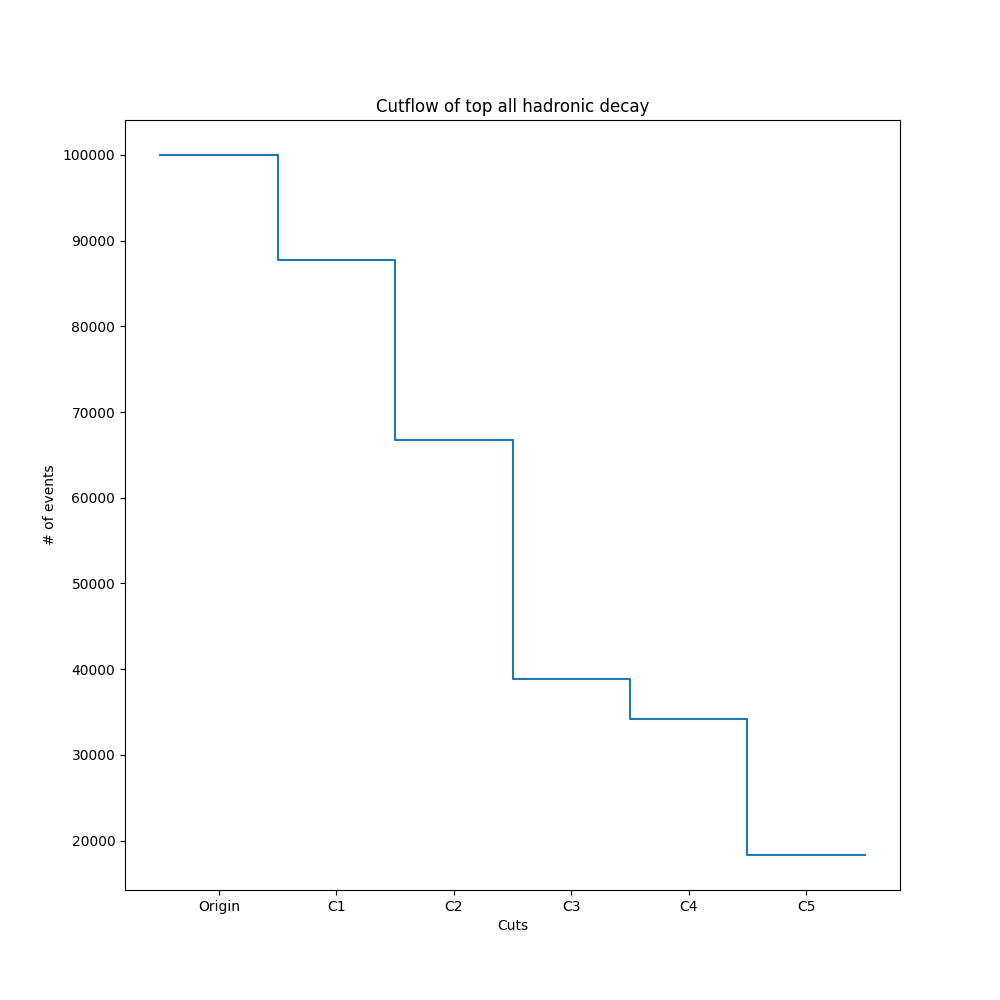
\includegraphics[width=0.8\linewidth, height=7cm,keepaspectratio=true]{Figures/ttbar_cutflow.png}
	\caption{Cutflow of all hadronic top decay.}
	\label{fig:cutflow}
\end{figure}
\begin{figure}[H]
	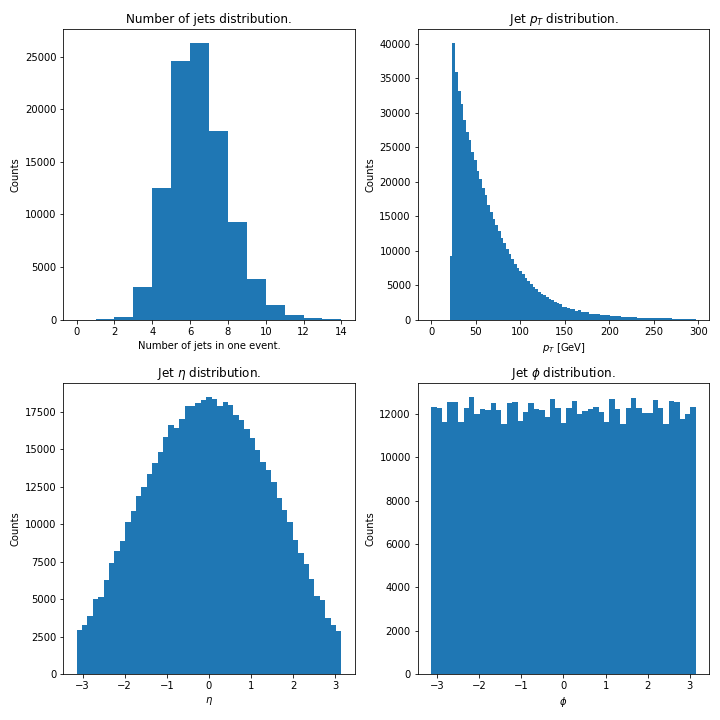
\includegraphics[width=0.8\linewidth, height=8cm,keepaspectratio=true]{Figures/ttbar_kinematic_dist.png}
	\caption{Demonstration of distributions.}
	\label{fig:kinematic dist}
\end{figure}
\newpage

\subsection{Truth matching}\label{subsec:Truth matching}
The \textbf{truth matching}, which is also called \textbf{$\Delta$R matching},  is to match the detector simulation(i.e. jet information generate by Delphes) data to truth record(i.e. Parton level information).  To calculate the $\Delta R$ value, we will find the daughters of top quarks, W boson, and b quark. After the daughters of top quarks are found, we will find the daughters of W bosons. Finally, we will get six partons that come from the decay of top quark pairs. These six partons can match the jets identically by considering their distances. The formula of calculating $\Delta R$ is:

\begin{equation}
	\Delta R = \sqrt{\Delta\eta^{2} + \Delta\phi^{2}}
\end{equation}
By using the kinematic properties provide in parton level and detector simulation information, we can calculate the $\Delta R$ value between each parton and jets. Using the result of the calculation, we may assign each parton to a specific jet. 

\subsection{Custom barcode system}\label{subsec:barcode}
To specify the relation between each parton, and the relation between mothers and daughters, we design a barcode system that helps us to declare the relationship.

\begin{figure}[h!]
	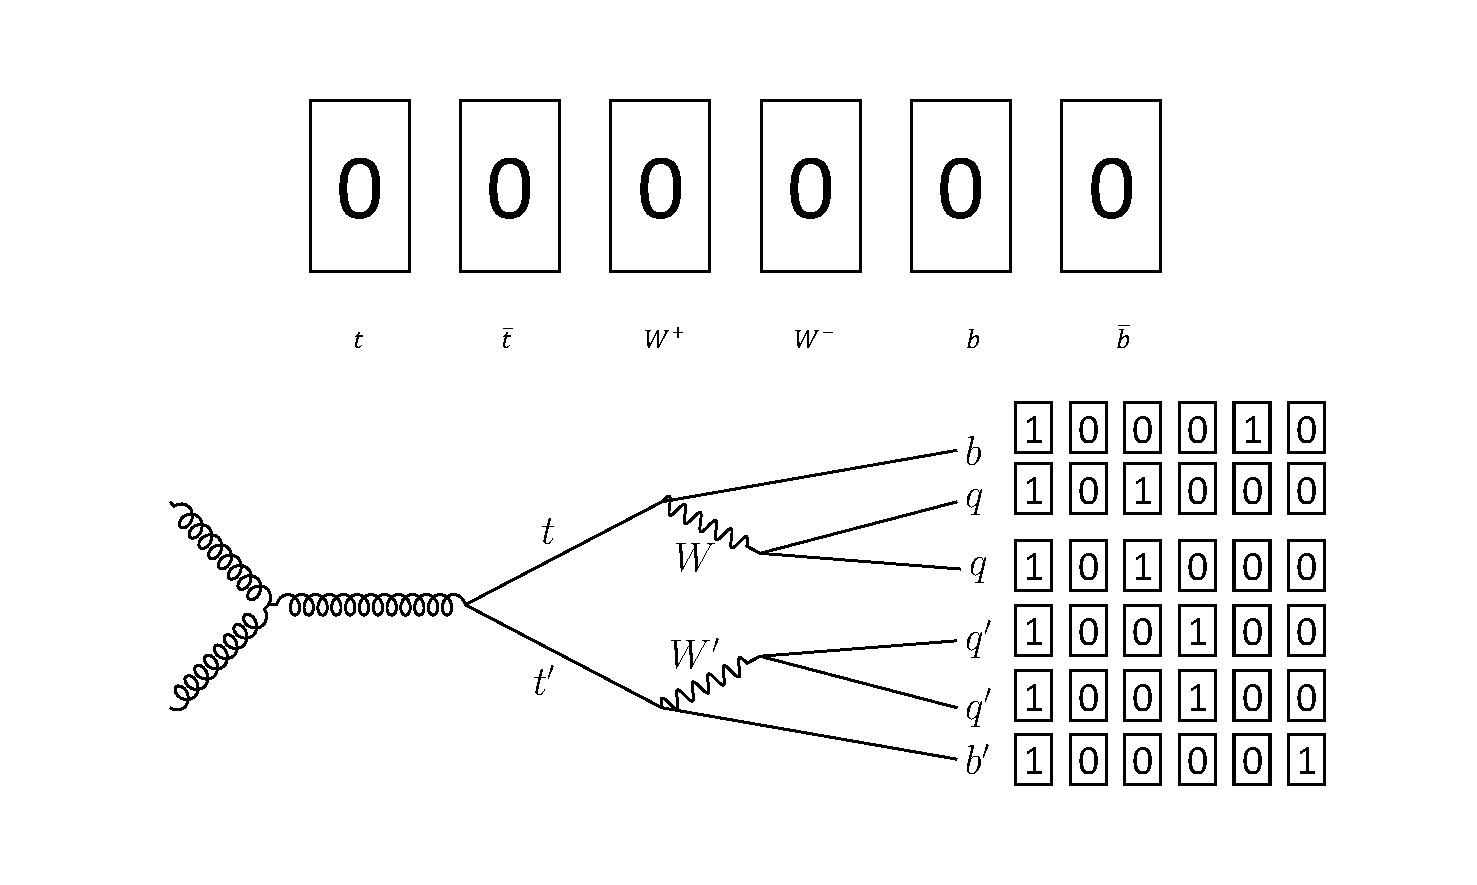
\includegraphics[width=0.8\linewidth]{Figures/barcode.pdf}
	\caption{Design of barcode.}
	\label{fig:barcode}
\end{figure}

In Figure \ref{fig:barcode}, we define a six-digit barcode, the first two digits are to show which top quark is the mother of this parton, the last four digits of the sequence is to declare which daughter of the top quark is the mother of parton. In case, we can use this barcode system to break six parton(jet) candidates into two subsets which contains 3 elements. The benefit of using this barcode system is not only can specify the relation without losing the information, but also provide a permutation relationship to our network. We will discuss this in the following section.

\section{Event reconstruction}\label{sec:Event reconstruction}

\subsection{$\chi^{2}$ reconstruction}\label{subsec:chi-square}

\subsection{Machine Learning Approach}\label{subsec:ML approach}


%Section \ref{subsec:data_trigger} discusses the triggers used, the trigger efficiencies and the gains of signals with the current setup.
%\section{Common event selection}\label{VBF:CommonSelection}
...

%\begin{itemize}
%	\item Exactly two opposite charged and different flavor leptons ($e\mu+\mu e$)
%	\item $\pTlead > 22$ \gev, $\pTsublead > 15$ \gev
%	\item $\mll > 10$ \gev
%\end{itemize}



%\begin{table}[!h]
%	\centering
%	\caption{Ranking of the BDT training variables \cite{ATLASComNote}.}
%	\label{tab:ranking}
%	\scalebox{0.8}{
	%	\input{Figures/VBFAnalysis/BDTInput/ranking.tex}
%	}
%\end{table}



%\begin{table}[!h]
%	\centering
%	\caption{ 
	%	Event yields in the VBF SR after fitting. Event yields in the highest BDT bin are also presented. The uncertainties include systematic and statistical uncertainties \cite{HWWRun2Paper}.}
%	\label{tab:ggF_VBF_yields}
%	\scalebox{0.8}{
	%	\input{Figures/Cutflow/VBFanalysis/EventYieldVBF.tex}
%	}
%\end{table}




